\documentclass{sig-alternate}

\usepackage{packages}

\newcommand{\sharedaffiliation}[0]{\end{tabular}\\\begin{tabular}{c}}

\title{Bug Isolation via Remote Program Sampling
  %%
  \thanks{This research was supported in part by NASA Grant
    No. NAG2-1210; NSF Grant Nos. EIA-9802069, CCR-0085949,
    ACI-9619020, and IIS-9988642; DOE Prime Contract No. W-7405-ENG-48
    through Memorandum Agreement No. B504962 with LLNL; and a Lucent
    GRPW Fellowship.  The information presented here does not
    necessarily reflect the position or the policy of the Government
    and no official endorsement should be inferred.}}

\numberofauthors{2}

\makeatletter
\newcommand*{\eecsMark}[0]{\@fnsymbol{2}}
\newcommand*{\statMark}[0]{\@fnsymbol{3}}
\makeatother
\newcommand*{\eecs}[0]{\textsuperscript{\eecsMark}}
\newcommand*{\stat}[0]{\textsuperscript{\statMark}}
\newcommand*{\both}[0]{\textsuperscript{\eecsMark, \statMark}}

\author{%
  %%
  \alignauthor Ben Liblit \eecs \\ \mailto{liblit@cs.berkeley.edu}
  \alignauthor Alex Aiken \eecs \\ \mailto{aiken@cs.berkeley.edu}
  %%
  \sharedaffiliation
  \alignauthor Alice X. Zheng \eecs \\ \mailto{alicez@cs.berkeley.edu}
  \alignauthor Michael I. Jordan \both \\ \mailto{jordan@cs.berkeley.edu}
  %%
  \sharedaffiliation
  \affaddr{\eecs Department of Electrical Engineering and Computer Science} \\
  \affaddr{\stat Department of Statistics} \\
  \affaddr{University of California, Berkeley} \\
  \affaddr{Berkeley, CA 94720-1776}}

\bibliographystyle{abbrv}

\begin{document}

\toappear{}
\maketitle

\begin{abstract}
We propose a sampling infrastructure for gathering information about
software from the set of runs experienced by its user community, and
show how to gather random samples with very low overhead for users.
Several example applications illustrate ways to use sampled
instrumentation to isolate bugs.  Assertion-dense code can be
transformed to share the cost of assertions among many users.  Lacking
assertions, broad guesses can be made as to crash-predictive program
behavior, and a process of elimination used to whittle these down to
the true bug.  Finally, even for non-deterministic bugs such as memory
corruption, a statistical modeling scheme based on logistic regression
allows us to identify program behaviors which are strongly correlated
with failure and where are therefore likely places to look for the
error.
\end{abstract}


\section{Introduction}

It is an unfortunate fact that almost all deployed software systems
have bugs, and that users often encounter these bugs.  For most
software, the resources (measured in time, money, or people) that can
be devoted to making improvements are limited, and the normal case is
that just through sheer numbers the user community brings far more
resources to bear on testing a piece of software than can be provided
by the team responsible for producing the software.

This paper is about making lemonade from lemons.  Given that deployed
software has problems, perhaps we can speed up the process of
identifying and eliminating those problems by learning something from
the enormous number of executions performed by the software's user
community.  We propose an infrastructure where some information about
each user execution of a program is transmitted to a central database.
The data gathered from all executions is analyzed to extract
information that helps engineers find and fix problems more quickly.
In our view, such an infrastructure has several benefits:
\begin{itemize}
  
\item For deployed software systems, the number of executions in
  actual use dwarfs the number of executions produced in testing by
  orders of magnitude.  For many software systems today, essentially
  all of the information from actual executions is discarded, because
  there is no mechanism for feedback.  Retaining even a small portion
  of that information could be valuable.
  
\item Gathering information from all, or at least a representative
  sample, of user executions gives an accurate picture of how the
  software is actually used, allowing better decisions about how to
  spend scarce resources on modifications. In particular, bugs that
  affect a large number of users are a higher priority than bugs that
  are very rare.  This kind of information is almost impossible to
  obtain from anywhere other than actual user executions.
  
\item While our primary interest is in finding and fixing quality
  problems, information gathered from user executions could be useful
  for other purposes.  For example, software authors may simply wish
  to know which features are most commonly used.
  
\item Traditional user feedback about problems often involves a call
  from a relatively unsophisticated user to a perhaps only somewhat
  more sophisticated technical support center.  In a networked world,
  it is simply more efficient and accurate to gather this information
  automatically.
  
\item Many bugs sit on open bug lists of products for an extended
  period of time before an engineer is available to work on the bug.
  Automatically gathering data from user executions allows for
  automated analysis, without human intervention.  Thus, when an
  engineer is finally available to work on a problem, the results of
  automated analysis done in the interim may help the engineer to
  identify and fix the problem more quickly.
  
  \disregard{
  \item Based on the current state of automatic analysis, clients can
    be instructed to focus attention in data gathering on different
    aspects of the software.  For example, if there appears to be a
    problem with a particular function $f$, we may wish clients to
    disproportionately report information about $f$ for a period of
    time, to speed up the process of gathering enough data for
    analysis.}

\end{itemize}

The idea of gathering data from actual user executions is not new.
Commercial databases, for example, routinely produce extensive log
files, and the first action when a user reports a problem is to
inspect those logs.  Similarly, each flight of the Boeing 777
generates logs which are subsequently combed for signs of possible
problems.  There are many other similar examples in the world of
commercial software.

A more recent development is the result of ubiquitous Internet
connectivity.  Netscape/Mozilla, Microsoft, GNOME, and KDE have all
deployed automated, opt-in crash reporting systems.  These systems
gather key information about program state after a failure has
occurred: stack trace, register contents, and the like.  By sending
this information back to the development organization, the community
helps developers effectively triage bugs that cause crashes and focus
on the problems experienced by the most users.

We believe this is progress in the right direction, but we also
believe that existing approaches only scratch the surface of what is
possible when developers and users are connected by a network.  For
example, the crash-reporting systems do not gather any information
about what happened before the crash.  Trace information leading up to
the failure may contain critical clues to the actual problem.  Also,
crash reporting systems report no information for successful runs,
which makes it difficult to distinguish anomalous (crash-causing)
behavior from innocuous behavior common to all runs.  In general, the
information gathered by crash-reporting systems is not very
systematic, and in all feedback systems of which we are aware
(crash-reporting or otherwise) the subsequent data analysis is highly
manual.

We present one approach to systematically gathering information about
program runs from a large, distributed user community and performing
subsequent automatic analysis of that information to help in locating
bugs.  Initially, we believed that the interesting problem was the
analysis of the data, and that gathering the data was relatively
straightforward.  However, we discovered that designing a data
gathering infrastructure that would scale is non-trivial.  As a
result, this paper discusses mostly the design and implementation of
the system that gathers the data from user executions
(\autoref{sec:framework}). We do give a non-trivial example of
subsequent data analysis in \autoref{sec:applications}.

Our infrastructure is designed to gather information about a large
number of program executions taking place remotely from a central site
where data is collected.  Any such design must solve two critical
problems.

The first problem is that the method for gathering information must be
sufficiently lightweight that it has a negligible impact on the
performance of the user's program.  Our approach, discussed in
\autoref{sec:framework}, is based on sampling.  Classical sampling for
measuring program performance searches for the ``elephant in the
haystack'': it is looking for the biggest consumers of time.  In
contrast, we are looking for needles (bugs) that may occur very
rarely, and furthermore our sampling rates may be very low to maintain
client performance.  This leads us to be concerned with guaranteeing
that the sampling is statistically fair, so that we can rely on the
reported frequencies of rare events.  We also develop new ways to
reduce the overhead of the necessary additional code that determines
whether to take a sample or not.

The second problem is that information from the client must be
transmitted over the network to the central database.  Generating
traces, or even partial traces, is simply too expensive in network
bandwidth even in cases where the performance impact on the client is
negligible.  Furthermore, gathering a relatively small amount of data
periodically from a large number of clients can quickly overwhelm the
storage capacity of a central server.  In our experience, compression
of the data must always be designed in to the analysis; we discuss
this further in \autoref{sec:applications}.

\autoref{sec:applications} presents two different applications of our
framework.  In \autoref{sec:share} we consider how we can share the
cost of program assertions over a large user base through sampling.
Each user only executes a fraction of the assertions, and thus sees
good performance, but in the aggregate bugs due to assertion failures
are still extremely likely to be detected.  In \autoref{sec:debug} we
show how we can use statistical techniques to identify the source of a
likely bug from samples taken from a few thousand executions.  We
sample information on the relationship between pairs of integer
variables in a program from both successful and failing runs and use
statistical regression techniques to identify those predicates that
are highly predictive of program failure.

Finally, monitoring of user executions raises some important privacy
and security concerns.  The problems are both social and technical; a
discussion of these issues appears in \autoref{sec:privsec}.

%% LocalWords:  privsec

\section{Sampling Framework}
\label{sec:framework}

This section describes our sampling framework.  We begin with sampling
of basic blocks and gradually add features until we can describe how
to perform sampling for entire programs.  Suppose we start with the
following C code:

\begin{code}
  check(p !=\ NULL); \\
  \up p = p->next; \\
  \\
  check(i < max); \\
  \up total += sizes[i];
\end{code}

Our sampling framework can be configured to sample arbitrary pieces of
code, which may be either portions of the original program or
instrumentation predicates added separately.  For this particular
example, assume that the italicized \texttt{\textit{check()}} calls
have been tagged for sampling.  A \texttt{\textit{check()}} call might
conditionally halt the program (as with \texttt{assert()}), or it
might append an event to a trace stream, or it might update a
per-predicate counter to record how often the predicate is true.  The
precise behavior of the instrumentation code is of no concern to the
sampling transformation itself.

\subsection{Sampling the Bernoulli Way}

Suppose that we wish to sample one hundredth of these checks.
Maintaining a global counter modulo one hundred is simple, but has the
disadvantage of being trivially periodic.  If the above fragment were
in a loop, for example, one of the checks would execute on every
fiftieth iteration while the other would never execute.  We wish
sampling to be fair and uniformly random: each check should
independently have a \nicefrac{1}{100} chance of being sampled each
time it occurs.  This is a so-called \termdef{Bernoulli process}, the
most common example of which is repeatedly tossing a coin.  We wish to
sample based on the outcome of tossing a coin which is biased to come
up heads only one time in a hundred.

A \naive approach would be to use a simple random number generator.
Suppose \texttt{rnd($n$)} yields a random integer uniformly
distributed between 0 and $n-1$.  Then the following code gives us
fair random sampling at the desired density:

\begin{code}
  if(rnd(100) == 0) check(p != NULL); \\
  \up p = p->next; \\
  \\
  if(rnd(100) == 0) check(i < max); \\
  \up total += sizes[i];
\end{code}

This strategy has some practical problems.  Random number generation
is not free: tossing the coin may be slower than simply doing the
check unconditionally.  Furthermore, what was previously straight-line
code is now dense with branches and joins, which may impede other
optimizations.

Sampling is sparse.  Each of the conditionals has a \nicefrac{99}{100}
= 99\% chance of not sampling.  On any run through this block, there
is a $(\nicefrac{99}{100})^2 \approx 98\%$ chance that both
instrumentation sites are skipped.  If we determine, upon reaching the
top of a basic block, that no site in that block is sampled, then we
can branch into fast-path code with all conditionally-guarded checks
removed.  This requires two versions of the code: one with sampled
instrumentation, one without.  It also requires that we can predict
how many future sampling opportunities are skipped before the next one
is taken.

Anticipating future samples requires a change in randomization
strategy.  Consider a sequence of biased coin tosses, with ``0''
indicating no sample and ``1'' indicating that a sample is to be
taken.  Temporarily increasing the sampling density to
\nicefrac{1}{5}, we might have:
%%
\begin{equation*}
  \langle
  \underbrace{0, 0, 0, 0, 0, 1}_6,
  \underbrace{0, 0, 0, 1}_4,
  \underbrace{0, 1}_2,
  \underbrace{0, 0, 1}_3,
  \dots
  \rangle
\end{equation*}

An equivalent representation counts the number of tosses until (and
including) the next sampled check: $\langle6, 4, 2, 3, \dots \rangle$.
This representation is predictive: the head of the sequence can be
treated as a countdown, telling us how far away the next sample is.
If we are at the top of a basic block containing only two checks, and
the next sampling countdown is 6, we know in advance that neither of
those sites is sampled on this visit.  Instead, we merely discard two
tosses and proceed directly to the instrumentation-free fast path:

\begin{code}
  if(countdown > 2) \{ \\
  \> /* fast path: no sample ahead */ \\
  \> countdown -= 2; \\
  \> \up p = p->next; \\
  \> \up total += sizes[i]; \\
  \} else \{ \\
  \> /* slow path: sample is imminent */ \\
  \> if(countdown-- == 0) \{ \\
  \>\> check(p != NULL); \\
  \>\> countdown = getNextCountdown(); \\
  \> \} \\
  \> \up p = p->next; \\
  \> \\
  \> if(countdown-- == 0) \{ \\
  \>\> check(i < max); \\
  \>\> countdown = getNextCountdown(); \\
  \> \} \\
  \> \up total += sizes[i]; \\
  \}
\end{code}

The instrumented code does extra work to manage the
next-sample countdown, but the fast path is much improved.  The only
overhead is a single compare/branch and a constant decrement, and this
overhead is amortized over the entire block.  In larger blocks with
more instrumentation sites, the initial countdown check has a larger
threshold, but that one check suffices to predict a larger number of
skipped sampling opportunities.

Consider the distribution of countdown values.  With a sampling
density of \nicefrac{1}{100}, there is a \nicefrac{1}{100} chance that
we sample at the very next opportunity.  There is a
$(\nicefrac{99}{100}) \times (\nicefrac{1}{100})$ that the next chance
is skipped but that the one after that is taken.  A countdown of three
appears on a $(\nicefrac{99}{100})^2 \times (\nicefrac{1}{100})$
chance, and so on.  These numbers form a \termdef{geometric
  distribution} whose mean value is the inverse of the sampling
density (that is, 100).  Numbers in a geometric distribution
characterize the expected inter-arrival times of a Bernoulli process.
However, repeated tossing of a biased coin is not necessary:
geometrically distributed random numbers can be generated directly
using a standard uniform random generator and some simple
floating-point operations.\footnote{In theory, a countdown may need to
  be arbitrarily large.  However, the odds of a \nicefrac{1}{100}
  countdown exceeding $2^{32}-1$ are less than one in $10^{10^7}$.}

As can be seen in the instrumented slow path, the countdown is reset
once it reaches zero.  Thus, we consume next-sample countdowns
gradually over time.  However, the rate of consumption is slower than
that for raw coin tosses: $n$ countdowns for $\nicefrac{1}{d}$
sampling encode, on average, $nd$ tosses.  A bank of pre-generated
random countdowns, then, is quite reasonable and will exhaust or
repeat $d$ times more slowly than would a similar bank of raw coin
tosses.

\subsection{From Blocks to Functions}

The scheme for blocks outlined above generalizes to an arbitrary
control flow graph as follows.  Any region of acyclic code has a
finite number of possible paths.  Let the maximum number of
instrumented sites on any path be the \termdef{weight} of that region.
If the next-sample countdown exceeds the weight of an acyclic region,
then no samples are taken on this pass through that part of the
code.  We can place a countdown threshold check at the top of this
region.

Cycles without instrumentation are effectively weightless and may be
disregarded.  A cycle with instrumentation must also contain a
threshold check.  This guarantees that if we start at any threshold
check and execute forward, we cross only a finite number of
instrumentation sites before reaching the next threshold check.  Thus,
we can compute a finite weight for each threshold check.

There is some flexibility regarding exactly where a threshold check is
placed; an optimal solution here is NP-hard
\cite{Hirzel:2001:BT-FLOTP}.  For simplicity, our present system
places one threshold check at function entry and one along each loop
back edge.  Weights may be computed in a single bottom-up traversal of
each function's control flow graph.  If any threshold check is found
to have zero weight, it is simply discarded.

We produce two complete copies of the function body.  One contains
full instrumentation, with each possible sample guarded by a decrement
and test of the next-sample countdown.  The other copy, the fast path,
merely decrements the countdown where appropriate, but otherwise has
all instrumentation removed.  We stitch the two variants together at
threshold check points: at the top of each acyclic region, we decide
whether a sample is imminent.  If it is, we branch into the
instrumented code.  If the next sample is far off, we continue in the
fast path code instead.

\begin{figure}
  \centering
  %% -*- LaTeX -*-

\CompileMatrices
\xymatrix@=10pt@d{
  &
  &
  *++[o][F.]{} \ar[r] &
  *++[o][F]{} \ar[r] &
  *++[o][F]{} \ar[rr] \ar[dr] &
  &
  *++[o][F.]{} \ar[r] &
  *++[o][F]{} \ar[r] \ar@(l,d)[llldd] &
  *++[o][F.]{} \ar[ddr] \\
  %%
  &
  &
  &
  &
  &
  *++[o][F.]{} \ar[ur] \\
  %%
  \ar[r]
  &
  *++[F-]{>4?} \ar[uur] \ar[ddr] &
  &
  &
  *++[F-]{>3?} \ar@(u,l)[uul] \ar@(u,r)[ddl] &
  &
  &
  &
  &
  \\
  %%
  \\
  %%
  &
  &
  *++[o][F.]{} \ar[r] &
  *++[o][F]{} \ar[r] &
  *++[o][F]{} \ar[rr] \ar[dr] &
  &
  *++[o][F.]{} \ar[r] &
  *++[o][F]{} \ar[r] \ar@(r,d)[llluu] &
  *++[o][F.]{} \ar[uur] \\
  %%
  &
  &
  &
  &
  &
  *++[o][F.]{} \ar[ur] \\
}


%% LocalWords: ur uur ddr ddl llluu llldd rr dr uul

  \caption{Example of instrumented code layout}
  \label{fig:code-layout}
\end{figure}

Figure~\ref{fig:code-layout} shows an example of code layout for a
function containing one conditional and one loop.  Dotted nodes
represent instrumentation sites; these are reduced to countdown
decrements in the fast path.  The boxed nodes represent threshold
checks; we have added one at function entry and one along the back
edge of the loop.  This code layout strategy is a variation on that
used by Arnold and Ryder to reduce the cost of code instrumented for
performance profiling \cite{Arnold:2001:FRC}.  The principal change in
our transformation is the use of geometrically distributed countdowns
in conjunction with acyclic region weights to choose between the two
code variants.  Arnold and Ryder use fixed sampling periods (e.g.,
exactly once per $n$ opportunities, or exactly once per $n$
instructions) and do not apply region-specific weighting.  Our
approach imposes more overhead, but offers greater statistical rigor
in the resultant sampled data.  Arnold and Ryder have studied several
variant layouts with varying trade-offs of code size versus overhead;
the same choices and trade-offs are directly applicable here.

\subsection{Function Calls}
\label{sec:framework:calls}

New optimization opportunities arise in the presence of function
calls.  A conservative treatment assumes any function call changes the
countdown arbitrarily.  Therefore, a new threshold check must appear
immediately after each function call.  This treatment is appropriate
if, e.g., the callee is being compiled separately.

However, if the callee is known and available for examination, a
simple interprocedural analysis can be used.  A \termdef{weightless
  function} has the following properties:

\begin{itemize}
\item The function contains no instrumentation sites.
\item The function only calls other weightless functions.
\end{itemize}

The set of weightless functions can be computed iteratively, requiring
no more steps in the worst case then the depth of the deepest
non-recursive call chain.

For purposes of identifying acyclic regions and placing threshold
checks, calls to weightless functions are invisible.  Acyclic regions
can extend below such calls, and no additional threshold check is
required after such a call returns.  A further benefit is that the
bodies of weightless functions may be compiled with no modifications.
They have no threshold checks, no instrumented code, and therefore
require no cloning or transformation of any kind.

\subsection{Global Countdown Management}

Our initial experience suggests that having the next-site countdown in
a global variable can be expensive.  Our system is implemented as a
source-to-source transformation for C, with \texttt{gcc} as our native
compiler.  We find that \texttt{gcc} treats the many
``\texttt{countdown--}'' decrements along the fast path quite poorly.
It will not, for example, coalesce a sequence of five such decrements
into a single ``\texttt{countdown -= 5}'' adjustment.  This apparently
stems from conservative assumptions about aliasing of global
variables.

Efficient countdown management requires that the native C compiler
take greater liberties when optimizing these decrements.  We assist
the native compiler by maintaining the countdown in a local variable
within each function:

\begin{enumerate}
\item At function entry, \termdef{import} the current global countdown
  into a local variable.
\item Use this local copy for all decrements, threshold checks, and
  sampling decisions.
\item Just before function exit, \termdef{export} this local copy back
  out to the global.
\end{enumerate}

To maintain agreement across all functions, we must also
export just before each function call and import again after each call
returns.  Again, though, calls to weightless functions may simply be
ignored, as they do not change or even inspect the countdown.
Similarly, the bodies of weightless functions need not import and
export at entry and exit, since they always leave the countdown
unchanged.  With this change, the conventional native C compiler can
coalesce decrements and perform other standard but important
optimizations.

\subsection{Issues in Remote Sampling}
\label{sec:compression}

Our framework for statistically fair sampling can be used for any
program monitoring application.  As discussed in
Section~\ref{sec:introduction}, there are issues peculiar to
monitoring a large number of remote sites.  Here we briefly discuss
the main problems and a particular solution that we adopt.

There are several dimensions in which performance can be harmed by
remote monitoring.  As usual the performance penalty imposed by the
extra monitoring code is a concern, but so are the use of local
storage to hold results (even temporarily) on a user's machine, the
use of network bandwidth to transmit results, and finally the storage
needed to hold results on a central server for analysis.  For example,
if we wish to retain all sampled data, then the storage requirements for the
central server grow linearly with the number of executions even if the
data collected from each execution is constant size.  
%In
%Section~\ref{sec:ccured} we give an example of an analysis that does
%not require retention of the data on the server.  However, we expect
%it will often be desirable to be able to perform a new analysis on
%previously gathered data and in this situation at least some data
%would need to be retained.

Our approach is to sample the number of observations of each of a very
large, but fixed, set of predicates (see Sections~\ref{sec:ccrypt}
and~\ref{sec:bc}).  The final form of the data is a vector of
integers, with position $i$ containing the number of times we observed
that the $i$th predicate was true.  For example, a typical entry might
be that the predicate $x > y$ at a particular program point was
observed to be true 42 times in one execution.

Maintaining a vector of counters produces data for an execution whose
size is largely independent of the sampling density or running time.
The loss of information, however, is significant, as the order
of the observations is discarded.  While our results can be interpreted
as showing that one can go a long way ignoring ordering, we expect
there are interesting applications that require ordering information.
We leave the problem of determining how to efficiently gather, store and
analyze partial traces (with ordering information) as future work.

%% LocalWords: rnd getNextCountdown pre

\section{Applications and Experiments}
\label{sec:applications}

We have used the transformation framework to inject different forms of
instrumentation into several programs, both to assess the performance
impact of sampling as well as to show that sampling can offer novel
insights into program (mis)behavior.

\subsection{Sharing the Cost of Assertions}
\label{sec:ccured}

In conventional usage, C \texttt{assert()} calls are used during
program development but are disabled (``\texttt{-DNDEBUG}'') when the
code ships to boost performance.  However, deployed programs fail in
unanticipated ways, and it would be helpful to retain some level of
assertion checking if the performance penalty were not excessive.

Programs produced by the \CCured instrumenting translator
\cite{POPL_'02*128} are extreme examples of assertion-dense code.
\CCured analyzes programs written in C and attempts to prove,
statically, that most pointer operations are memory safe.  Where this
cannot be done, \CCured inserts dynamic checks to enforce memory
safety at run time.  For purposes of our research, \CCured is simply a
source of highly assertion-dense code.  The individual assertions are
quite small and fast: array bounds checks, testing for null, etc.
However, in large numbers, their performance impact can be
considerable.  We wish to use random sampling to spread this cost
among many users.

We have applied sampling to several benchmarks taken from the Olden
\cite{Carlisle:1996:OPPWDDSDMM} and SPECINT95 \cite{SPEC95} benchmark
suites.  All programs run to completion and we are simply measuring
the overhead of performing the dynamic checks.

\subsubsection{Whole-Program Sampling}
\label{sec:share:whole}

\begin{table*}[tb]
  \centering
  \small
  \begin{tabular}{|l|rrr|rrr|}
    \hline
    & \multicolumn{3}{c|}{\textbf{function counts}} & \multicolumn{3}{c|}{\textbf{average for functions with sites}} \\
    \raisebox{1.5ex}[0pt]{\textbf{benchmark}} & \textbf{total} & \textbf{weightless} & \textbf{has sites} & \textbf{sites} & \textbf{threshold checks} & \textbf{threshold weight} \\
    \hline\hline
    \texttt{bh} & 64 & 15 & 48 & 11.9 & 3.8 & 9.5 \\
\texttt{bisort} & 13 & 3 & 10 & 4.1 & 1.9 & 2.6 \\
\texttt{em3d} & 15 & 5 & 10 & 5.5 & 3.1 & 4.7 \\
\texttt{health} & 16 & 2 & 14 & 6.1 & 2.9 & 3.1 \\
\texttt{mst} & 16 & 5 & 11 & 6.2 & 2.5 & 3.9 \\
\texttt{perimeter} & 11 & 4 & 6 & 7.8 & 2.7 & 2.1 \\
\texttt{power} & 19 & 4 & 15 & 5.8 & 3.0 & 2.8 \\
\texttt{treeadd} & 7 & 2 & 5 & 3.6 & 2.0 & 2.5 \\
\texttt{tsp} & 14 & 5 & 8 & 15.2 & 3.9 & 3.5 \\
\hline
\texttt{compress} & 20 & 4 & 15 & 7.1 & 2.9 & 3.9 \\
\texttt{go} & 380 & 12 & 359 & 14.8 & 6.0 & 4.7 \\
\texttt{ijpeg} & 314 & 34 & 267 & 18.7 & 5.0 & 7.3 \\
\texttt{li} & 375 & 16 & 336 & 6.2 & 3.2 & 2.9 \\
\hline

  \end{tabular}
  \caption{Static metrics for \CCured benchmarks.  Olden benchmarks
    are listed first, followed by SPECINT95.}
  \label{tab:share:static}
\end{table*}

\autoref{tab:share:static} summarizes static aspects of the sampling
transformation when applied to the entirety of each benchmark.  For
each program, we give the total number of non-library functions and
the number of these that are weightless.  \CCured is a whole-program
analysis, so weightless function identification has the advantage of
being able to examine every function body.  We also count the number
of functions which directly contain at least one instrumentation site.
(What remains are those functions which contain no sites of their own
but which call other functions that do have sites.)

Considering just the functions which directly contain at least one
instrumentation site, \autoref{tab:share:static} also presents the
average number of sites per function, the average number of threshold
check points per function, and the average threshold weight for all
such points.  (Note that the product of the last two of these metrics
may exceed the first, as a single instrumentation site may fall under
more than one threshold check point.  This can be seen in the example
in \autoref{fig:code-layout} as well.)  The average site count gives
an impression of how assertion-dense the code is.  The average
threshold weight measures how effective our transformation has been in
amortizing the cost of countdown checks over multiple sites.
Single-site functions are not uncommon; thus, an average threshold
weight above two is encouraging because it suggests that overall
amortization rates are fairly good.

\begin{table}
  \centering
  \begin{tabular}{|l|r|rrrr|}
    \hline
    \rule{0pt}{2.5ex}
    \textbf{benchmark} & \textbf{always} & $\mathbf{10^{-2}}$ & $\mathbf{10^{-3}}$ & $\mathbf{10^{-4}}$ & $\mathbf{10^{-6}}$ \\
    \hline\hline
    \texttt{bh} & 2.81 & \textit{1.30} & \textit{1.10} & \textit{1.07} & \textit{1.07} \\
\texttt{bisort} & 1.08 & \textit{1.07} & \textit{1.05} & \textit{1.05} & \textit{1.04} \\
\texttt{em3d} & 2.14 & \textit{1.12} & \textit{1.04} & \textit{1.02} & \textit{1.04} \\
\texttt{health} & 1.02 & 1.03 & \textit{1.02} & \textit{1.02} & \textit{1.02} \\
\texttt{mst} & 1.25 & \textit{1.06} & \textit{1.04} & \textit{1.03} & \textit{1.04} \\
\texttt{perimeter} & 1.08 & 1.19 & 1.13 & 1.13 & 1.12 \\
\texttt{power} & 1.36 & \textit{1.07} & \textit{1.05} & \textit{1.04} & \textit{1.04} \\
\texttt{treeadd} & 1.13 & \textit{1.09} & \textit{1.09} & \textit{1.09} & \textit{1.11} \\
\texttt{tsp} & 1.05 & 1.17 & 1.16 & 1.15 & 1.14 \\
\hline
\texttt{compress} & 2.01 & \textit{1.21} & \textit{1.14} & \textit{1.14} & \textit{1.14} \\
\texttt{go} & 1.17 & 1.46 & 1.26 & 1.22 & 1.22 \\
\texttt{ijpeg} & 2.46 & \textit{1.17} & \textit{1.05} & \textit{1.04} & \textit{1.03} \\
\texttt{li} & 1.58 & \textit{1.24} & \textit{1.18} & \textit{1.16} & \textit{1.16} \\
\hline

  \end{tabular}
  \caption{Relative performance of various sampling rates versus no
    instrumentation.  \textit{Italics} marks cases where sampled
    instrumentation outperforms unconditional instrumentation.}
  \label{tab:share:density}
\end{table}

\autoref{tab:share:density} shows the performance effect of various
sampling densities.  We take the running time of standard \CCured code
as the baseline.  We report the speedup ($>1$) or slowdown ($<1$)
relative to this baseline when sampling at various densities.  All
benchmarks were compiled using \texttt{gcc} 2.96 using standard
optimization (\texttt{-O2}).  Times were collected on a 550 MHz
Pentium III Linux machine with two gigabytes of RAM\@.  Reported
speedups represent the average of four runs; each run used a different
pre-generated bank of 1024 geometrically distributed random
countdowns.

Even at a fairly high sampling density of 1/100, more than two thirds
of our benchmarks run faster then they would if all checks were
performed.  Because each single check is so small and fast, this
suggests that we have been successful in amortizing our sampling
overhead.  The most dramatic speedups are seen in \texttt{ijpeg} (24\%
faster) and \texttt{compress} (32\% faster).  On the other hand, three
benchmarks do run slower, with \texttt{go} showing the largest
penalty.  In these cases, the time recovered by skipping 99/100 checks
is not enough to mask the added overhead of sampling.

As we reduce the sampling density to 1/1000, \texttt{power} reaches a
balance point of no measurable speedup or slowdown, while
\texttt{perimeter} remains a stubborn 3\% slower.  The \texttt{health}
benchmark crosses over and is now slightly faster with sampling.
Other benchmarks, which already showed speedups at 1/100, either
retain their position (\texttt{treeadd} and \texttt{tsp}) or show
additional boosts, with \texttt{compress} reaching an overall 38\%
speedup versus standard \CCured.  Further reducing the sampling
density to 1/10,000 shows little change, and by the time we reach
1/1,000,000 it is clear that we have reached a performance ceiling.
One benchmark continues to run slower than standard \CCured; two run
at the same speed; the remaining ten run 2\% - 39\% faster.

\subsubsection{Single-Function Sampling}
\newcommand{\execGrowthMin}{9}
\newcommand{\execGrowthMax}{78}


In an effort to better understand the sources of overhead, we have
performed additional experiments in which only a single function is
instrumented at a time.  This also approximates a more realistic
approach to managing code size.  The fully instrumented executables
from \autoref{sec:share:whole} range from
\execGrowthMin\%-\execGrowthMax\% larger than their non-sampling
counterparts.  When only a single function is instrumented, code
expansion is small enough to not be a concern.

A fully deployed system might use dynamic instrumentation to randomly
instrument a single selected function \textit{du jour}.  For the
present research, we build one executable for each site-containing
function as counted in \autoref{tab:share:static}.  All sites in other
functions are removed.  This, in turn, allows us to discover many more
weightless functions: any function which cannot transitively call the
one function being instrumented is weightless.  Thus, a suite of
single-function sampling executables may perform better, over all,
than a single executable with sampling in all functions.

\begin{figure}
  \centering
  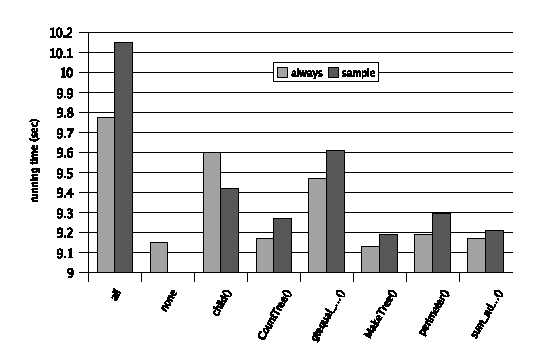
\includegraphics[width=\columnwidth]{applications/perimeter}
  \caption{\texttt{perimeter} running times with single-function
    instrumentation}
  \label{fig:share:perimeter}
\end{figure}

In the interest of space, we report only on \texttt{perimeter}: the
stubborn worst performer from the preceding experiment.  This
benchmark's small function count also makes overall results easier to
visualize.  \autoref{fig:share:perimeter} shows absolute running times
in seconds, with 1/100 sampling.  The two leftmost ``all'' bars
represent instrumenting all functions, either with checks always done
or with checks sampled.  The solo ``none'' bar represents the extreme
limit of performance: all instrumentation statically removed from all
functions.  No instrumentation scheme, with or without sampling, can
run faster than this.  The remaining bars show the running time for
each site-containing function, with that function's sites either
checked always or sampled 1/100.

Note that the vertical baseline is nine seconds, not zero, which
magnifies fairly small differences: the two leftmost bars differ by
only 4\%, the same difference reported in the ``$10^{-2}$'' column for
\texttt{perimeter} in \autoref{tab:share:density}.

Among the site-containing functions, \texttt{child()} gains a small
performance boost from sampling.  The remaining five are all
self-recursive, with between one and four recursive calls.  Our
current system treats each of these as a call to a non-weightless
function: the countdown must be exported before the call and imported
after.  A faster approach would be to transform each function to pass
the local countdown down to its recursive callees, and accept an
updated countdown back as a returned value.  Such a countdown
management strategy would be applicable any time both callee and
caller can agree on the API change; the case of self-recursive calls
is particularly straightforward.  It is worth noting that
\texttt{child()}, which does show sampling speedup, is the only
function of these six which is not self-recursive.

Benchmarks that are less dominated by recursion suggest additional
areas for improvement.  Recurring trends include:

\begin{itemize}
\item Low amortization due to lightweight regions in loops with bounds
  that are constant or fixed on entry.  A loop with iteration count
  $i$ and body weight $w$ could be treated as an acyclic region of
  weight $iw$.

\item Conservative identification of weightless functions.  Calls
  through function pointers or to externally-defined code are assumed
  to potentially recurse back to the caller.  Points-to analyses can
  improve the former; a statically checkable \texttt{weightless}
  annotation on function prototypes would resolve the later.
\end{itemize}

When multiple functions are being instrumented, we find another area
for improvement.  Some callees may not be weightless, but can never
cross more than some finite number of sites per call.  The caller of a
finite-weight function can exploit this upper limit, effectively
treating the callee as a cluster of sites of appropriate weight.

We expect that these and other optimizations will continue to improve
the performance benefit from sampling, both for single-function as
well as whole-program instrumentation.

\subsection{Bug Isolation Using Feature Elimination}
\label{sec:ccrypt}

%% \aside{Story to tell here:

%%   Preceding experiment is all well and good if possible failure points
%%   are explicitly marked with assertions, but you can't expect that in
%%   general.  Instead, we want to make fairly wild guesses about
%%   possible problems, then eliminate these in light of their behavior
%%   in actual runs.  Function return values are a good place to make
%%   these guesses, as they are often used to indicate success or failure
%%   of a given operation.  Experiment with \texttt{ccrypt} shows that we
%%   can reliably rediscover a known fatal error by sampling and
%%   filtering function return values.

%%   We didn't have the \texttt{ccrypt} experiment when we first wrote up
%%   the \texttt{bc} experiment, so \autoref{sec:bc} already spends
%%   some time introducing the idea of counter triples, randomized input
%%   to simulate a large user community, etc.  Some of that text should
%%   probably be lifted up and placed here instead.}


\CCured style bug-hunting techniques is all well and good if possible
failure points are explicitly marked with assertions.  But in general,
this is not to be expected.  Crafting potentially useful assertions is
at best a painstaking process; more often than not, it is horribly
ineffective.  In this and the next subsections, we describe how to
harness the power of thousands of trial users to cast a much bigger
net, one that leads to the automatic discovery of sometimes
non-trivial bugs.  First, a large number of fairly wild guesses about
possible problems are strewn into the code, their behavior at run time
is then sampled under the framework described in
\autoref{sec:framework}.  After collecting a number of these trial
runs, we combine simple rules and more sophisticated statistical
techniques to automatically eliminate swaths of wrong guesses, leaving
just a handful of guesses that accurately isolate the location of the
bug.

Function return values are good candidate guesses for where a bug may
hide.  Often times a program crashes because it has neglected to check
for the (failed) return value of a function call.  The compression
program \texttt{ccrypt} is a good example.  Given an input file, the
program first checks whether the designated output file exists; if
so, it asks the user whether or not to overwrite it.  The function
\texttt{xreadline()} returns the user response string, which is then
directly sent to \texttt{strcmp()} without checking for the validity
of the string pointer.  Hence if the user responds with \texttt{eof},
\texttt{xreadline()} will return the \texttt{NULL} pointer, causing the
program to crash in \texttt{strcmp()}.

The \texttt{ccrypt} bug is a deterministic one, meaning that without
exception, the program crashes if and only if \texttt{xreadline()}
returns zero or \texttt{NULL}.  This is different from the kind of
non-deterministic bugs often seen with memory corruption: sometimes
the bug will result in a crash, but occasionally the program completes
successfully even in the presence of the bug.  Additionally, the
\texttt{ccrypt} bug is very close to the actual crashing point, making
debugging very easy for a human.  Nevertheless, this kind of bug is an
annoyance in a large program with many other bug reports.  It also
poses a sanity check for the automatic bug-hunting approach: one
would hope that there is a very simple solution to catch these
simple deterministic bugs.  Our solution, as it turns out, does not
even require the heavy statistical machinery needed in
\autoref{sec:bc}; it is based on straightforward logical
reasoning.

Since we do not have ready access to thousands of users, we simulate
a large user community by using randomly generated inputs in the
spirit of the Fuzz project~\cite{MKLMMNS95}.  For each trial run, we
generate a random input file, and sometimes, we also generate an
output file in order to induce the crash.  Assertions are instrumented
into the code to compare every function call return value against zero
(the usual signal for success).  A direct trace of these comparisons
is out of the question: even with very sparse sampling, the
amount of data generated would overwhelm the client, network, and
server.  Instead, we locally reduce the trace by merely recording the
number of times the return value is greater than, less than, or equal
to zero.

For \texttt{ccrypt}, this results in 570 predicates, or $570 * 3 =
1710$ total number of counters.  In statistical analysis lingo, each
of these counters is a \termdef{feature}.  Only one of these features
is what we want, namely, the one of the return value of
\texttt{xreadline()} being equal to 0.  Our dataset contains 2990
trial runs at a sampling rate of $1/1000$; on average, the
program records the value of only one instrumentation site for every
thousand that it encounters.  This means that, with high probability,
we will not have sampled the return value of \texttt{xreadline()} for
any single run.  In fact, out of the 2990 trial runs, only 88
ultimately resulted in a crash, and the smoking gun is observed in
only one of these crashes.  But the picture is not quite as bad as it
may seem: shuffling through the data a bit, we notice that out of the
1710 counters, only 141 of them are ever non-zero.\footnote{Beyond
  simplifying the statistical analysis, this degree of regularity
  means that counter reports are highly compressible: good news for
  deployed users with small hard drives or slow modems.}  Still, this
poses a daunting task for any statistical analysis technique.

Let's stop for a bit and think about the problem rationally.  As a bug
hunter, we may have some intuition about the bug, or at least we can
try out several alternatives.  First, we can assume that the bug is
deterministic and see where that leads us.  Right away, this
assumptions means that a predicate that is true for any successful run
can never be the bug -- if it were, then the program would have
crashed.  Hence we can eliminate all the counters that are ever
non-zero in any of the 2902 successful runs, and only keep those
that are always zero for all successful runs. Doing this feature
elimination step on the 141 features leaves us with just 2 features,
one is the predicate for \texttt{file\_exists()} returning true ($>
0$), and the other the smoking gun.

The result is encouraging.  However, we may question whether using
close to 3000 trial runs to find one simple bug is an overkill.  More
importantly, we would like to know how many successful runs it takes
on average to weed out all but a handful of the ``good'' features,
i.e. those that are most likely bugs in the program.
\autoref{fig:ngood} plots the number of ``good'' features selected,
averaged across 100 random sequences of subsets of the 2902 successful
runs.  The crosses mark the means, while the vertical bars extend one
standard deviation above and below the mean.  The curve drops very
sharply with the first few hundred runs, and slowly peter out in the
tail.  The short vertical bars in this case tells us that there's not
much variation across the 100 random sequences of subsets.  The
results show that, on average, 650 runs are enough to isolate 20
candidate features, another 550 runs reduces that count by half, and
a total of 1750 runs is enough to narrow the set of good features down
to 5.

\begin{figure}
  \centering
  \small
  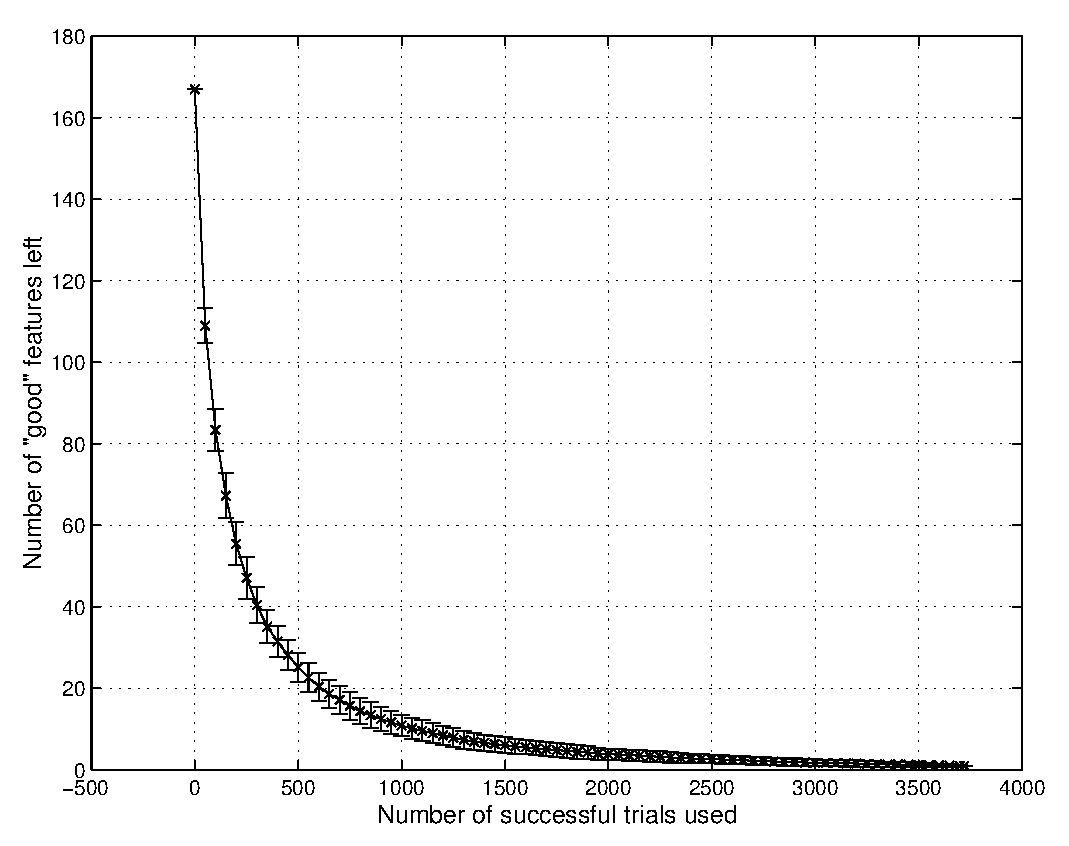
\includegraphics[width=\columnwidth]{applications/ds1000ngood_plot}
  \caption{Effect of dataset size on the number of good features
    selected by the all-zero-for-all-successes feature selection
    process.}
  \label{fig:ngood}
\end{figure}

In the field of statistical analysis and machine learning,
\termdef{feature selection} is a symmetric notion: important features
are those that are highly correlated with either crashes or successes.
However, when it comes to bug isolation, we only want the features
that are predictive of a crash.  We can make good use of this kind of
\termdef{negative information} in our analysis.  While we cannot
always be certain which ones are predictive of a crash, we can
eliminate those features that could not possibly have caused the
crash.  The zero-for-all-successes selection criterion that we
describe above lies along this line of reasoning.  However, it only
works if the bug is deterministic.  If there is are cases where
the program succeeds despite the occurrence of the bug, then the
criterion would wrongly eliminate the actual bug.

A rule that works for both sporadic and deterministic bugs is to
eliminate those features that are always zero in all the observed
crashes.  The reason is that predicates that are never observed to be
true in any crashes represent events that are never witnessed in
those crashes.  Assuming that we have enough crashed trial runs at the
given sampling rate to observe the event at least once, then a event
that was never observed in these trials could not possibly have caused
the crash.  Applying this rule to the 141 effective predicates of the
88 crashed runs leaves us with 45 features.

A third criterion is to eliminate those features representing lines of
code that were never reached due to the crash: un-executed code could
not cause a crash.  A rough count of code coverage can be obtained by
summing the triple counters for each predicate.  In the case of
\texttt{ccrypt}, summing the number of times a return value is greater
than, equal to, or less than zero, gives us the total number of times
we sampled that return value.  Again assuming we have enough number of
runs in our data set, if the sum is always zero, then with high
probability, the instrumentation site in question was probably never
reached during any crashed run.  Notice that the set of features
eliminated using this rule is a subset of those eliminated by rule two
above.  Counter values are always non-negative, hence if the sum of
the three counters is zero for all crashes, then each individual
counter must also be zero for all crashes.  Applying rule three to the
\texttt{ccrypt} crashed runs leaves us with 48 features, including the
45 that were selected by rule two.

We have already alluded to the combined effect of sampling rate and
dataset size on our confidence results.  More specifically, suppose we
are interested in an event that will happen exactly once during a
trial run.  At a sampling rate of $1/1000$, we'll observe this event
an average of once every thousand trials.  To be $95\%$ confident that
we'll have observed said event at least once, we'll need at least
$\log(1-0.95)/ \log(1-1/1000) \approx 2995$ trials.

In summary, the \texttt{ccrypt} example illustrates a simple bug that
can be rooted out using simple techniques.  There are three strategies
that we can use for feature elimination:
%%
\begin{enumerate}
\item[1.] discard a feature if it is nonzero in any successful run;
\item[2.] discard a feature if it is zero in every failed run;
\item[3.] discard a feature triple if their sum is zero in every failed run
\end{enumerate}
%%
Rule 1 cannot be used if the bug is suspected to be
non-deterministic.  Rule 2 in fact covers rule 3, but neither are as
effective for a deterministic bug.  In the next subsection, we look at
a more elusive bug and describe powerful statistical techniques used
to catch it.

\subsection{Statistical Debugging}
\label{sec:bc}

%% this paragraph no longer fits the flow here, perhaps we can make
%% this point elsewhere in the paper?  [axz]
%% Sampled information about program behavior can be thought of as a
%% database.  Data mining techniques, then, may reveal important
%% information about the aggregate behavior of many runs.  Of particular
%% interest to us is finding and fixing bugs.  We now illustrate how
%% mining of sampled program behavior can help direct software engineers
%% to the root cause of difficult bugs.

Our next target is version 1.06 of the GNU implementation of
\texttt{bc}.  We find that feeding \texttt{bc} nine megabytes of
random input causes it to crash roughly one time in four.
\disregard{While this would be an unusually high failure rate for
  shipping software under normal usage patterns, we expect that users
  experiencing crashes will be more likely to opt-in to a trace
  reporting system.  Thus, this may be a reasonable ratio to expect if
  most crashes and a few non-crashes are reported.}
Quick perusal of the stack trace at a typical failure is discouraging.
The crash occurs several frames deep inside the C library's
\texttt{malloc()} function: a sure sign of heap corruption.  Such bugs
are especially pernicious because the actual corruption may have
happened well before the ultimate crash \cite{Eisenstadt1993b}.

We instrument \texttt{bc} to guess and randomly check a large number
of possible invariants.  Our goal is to identify predicates that hold
when the program succeeds, but which are violated when the program
crashes.  We cast an extremely broad net, but with an eye toward
pointer use errors and buffer overruns.  For pointer use, null
pointers are clearly of interest.  Relative addresses of pointers may
be interesting as well, as this may capture cases where one pointer
scans within a second pointed-to buffer.  Checking pointer/pointer
equality may reveal aliasing which, when not anticipated by the
programmer, can lead to dangling ``wild'' pointer bugs.  Scalar
variables serve as array indexes, pointer offsets, and in many other
roles; relationships among scalars may reveal buffer overruns,
unanticipated consequences of negative values, invalid enumeration
constants, or a variety of other problems.

At any direct assignment to a scalar variable \texttt{a}, we identify
all other local or global variables $\{ \mathtt{b}_1, \mathtt{b}_2,
\dots, \mathtt{b}_n \}$ which are also in scope and which have the
same type.  We then compare the updated \texttt{a} to each
$\mathtt{b}_i$, and note whether \texttt{a} was less than, equal to,
or greater than $\mathtt{b}_i$.
%% the following sentence has been moved to the previous subsection [axz]
%% Even with very sparse sampling, a direct trace of these comparisons
%% would overwhelm both client, network, and server.  Instead, we
%% locally reduce the trace by merely counting how often each of the
%% three relative orderings appeared.
We compare pointers to same-typed pointers as well, and additionally
compare each pointer for equality with null.  One comparison between
\texttt{a} and $\mathtt{b}_i$, which bumps one of three counters, is
considered to be one instrumentation site subject to random sampling.
When an instrumented application terminates, it emits the vector of
counter triples along with a flag indicating whether it completed
successfully or was aborted by a fatal signal.

%% changed number of counter triples to reflect the dataset without
%% bison/lex lines
As expected, this gives us a large number of candidate predicates:
10,050 counter triples, or 30,150 counters in all.  Because our
guesses are so crude, the vast majority of these are of no interest:
either they compare completely unrelated variables, or they express
relationships which behave identically in both successful and failed
runs.  The challenge is to find those few candidate predicates which
truly matter.

\subsubsection{Crash Prediction Using Logistic Regression}

To find these few important predicates, we recast the bug hunt as a
statistical analysis problem.  Each run of \texttt{bc} constitutes one
sample point consisting of 30,150 observed \termdef{features} and one
binary \termdef{outcome} ($0 = \text{succeeded}, 1 = \text{crashed}$).
In C, a misbehaving program can sometimes ``get lucky'': it may
violate memory safety yet not crash.  Hence the outcome label is
non-deterministic.  Given numerous data points (sampled runs), we
would like to identify a narrow subset of our 30,150 features which
are relevant to predicting the succeeded/crashed outcome.  This is
equivalent to the machine learning problem of learning a binary
classifier with feature selection, i.e.\ using as few input features
as possible.

In the classification setting, we take a set of data with known binary
output (a training set), and attempt to learn a binary classifier that
gives good predictions on a test set.  The learning process usually
involves additional parameters whose values can be determined using a
validation set.  In our case, the end goal is to narrow down the set
of features.  Hence our method will have to balance good
classification performance with aggressive feature selection.

A binary classifier takes feature values as inputs, and outputs a
prediction of either $0$ or $1$.  \termdef{Logistic regression}
\cite{Hastie01} is a method of learning a binary classifier where the
output function is assumed to be logistic.  The logistic function is a
continuous ``S''-shaped curve approaching 0 on one end, and 1 on the
other.  The output can be interpreted as a probability measure of how
likely the data point falls within class 0 or 1.  Quantizing the
logistic function output then gives us a binary classifier: if the
output is greater than $1/2$, then the data point is classified as
class 1 (a crash), otherwise it falls under class 0 (a successful
run).  Feature selection can be achieved by \termdef{regularizing} the
function parameters to ignore most input features.

\aside{Alice writes: this paragraph should be revisited after we
  finish the experimental results.}

While other ways of combined classification and feature selection
exist, none of them are particularly well-suited for this problem.
Some methods \cite{Golub:MCC:1999,Tibshirani2002} calculate a
univariate correlation coefficient independently for each feature;
other methods, such as decision trees \cite{00000048}, are more
computationally intensive.  In our dataset, the features are clearly
not independent of each other, and the size of the problem can
potentially be too large for more computationally intensive methods.
Furthermore, logistic regression is a discriminative classification
method, and thus does not make any assumptions about the underlying
distribution of the input.  This is crucial since our features arise
from a decidedly artificial process and would be difficult to
characterize using simple distributions.

Suppose our training set $\mathcal{D}$ consists of $M$ data points
$(x_1,y_1), \ldots, (x_M, y_M) $, where each $x_i \in \Real^N$ denotes
a vector of input predicate counters, and each $y_i = \{0, 1\}$
denotes the corresponding output label.  To learn a good classifier,
we can maximize the \termdef{log likelihood} of the training set.
%%
\begin{equation*}
  \begin{split}
    LL(\mathcal{D}) \:=\:
    \sum_{i=1}^M \, [ & y_i \log P(Y = 1 | x) \\
    + & (1 - y_i) \log (1 - P(Y = 1 | x)) ]
  \end{split}
\end{equation*}
%%
Here the output labels $y_i$ are used as indicator functions to zero
out exactly one of the two terms in each summand.  In logistic
regression, the distribution $P(Y=1|x)$ is modeled as the logistic
function $\mu_{\tilde{\beta}}(x)$ with parameters $\tilde{\beta} = \langle \beta_0 \in
\Real, \beta \in \Real^N \rangle$.
%%
\begin{equation*}
  P(Y = 1 | x) = \mu_{\tilde{\beta}} (x) = \frac{1}{1 + \exp(- \beta_0 - \beta^T x)}
\end{equation*}
%%
The logistic parameters $\beta_0$ and $\beta$ take on the respective roles as
the intercept and slope of the classifier, and essentially weigh the
relative importance of each feature in the final outcome.  We expect
most of the input features to have no influence over the success or
failure of the program, so we place an additional constraint that
forces most of the $\tilde{\beta}$'s toward zero.  This is accomplished by
subtracting a penalty term based on the L1-norm $\norm{\tilde{\beta}}_1 =
\sum_{j=0}^M \abs{\beta_j}$.  We can tune the importance of this
\termdef{regularization term} through a \termdef{regularization
  parameter} $\lambda$.  The penalized log likelihood function is:
%%
\begin{equation*}
  \begin{split}
    LL (\tilde{\beta} | \mathcal{D}, \lambda ) \:=\:
    & \sum_{i=1}^M \, [y_i \log \mu_{\tilde{\beta}} (x_i) + (1 - y_i) \log (1 - \mu_{\tilde{\beta}} (x_i))] \\
    & - \lambda \norm{\beta}_1
  \end{split}
\end{equation*}
%%

\subsubsection{Bug Hunting in \texttt{bc}}
Our \texttt{bc} dataset consists of 4390 runs with distinct random
inputs and distinct randomized $1/1000$ sampling, of which 2729 are
randomly chosen for training, 322 for validation, and 1339 for
testing.  Although there are 30,150 raw features, many can be
discarded immediately: in the training set 27,242 features are always
zero.  Hence the effective number of features used in training is
2908.  (Applying rule 2 described in \autoref{sec:ccrypt} can
eliminate another 647 features that are zero for all failed runs.  But
the presence or absence of these 647 features turn out not to affect
the quality of the regularized logistic regression results.)
Furthermore, to make the magnitude of the $\beta$ parameters
comparable, the feature values have to be on the same scale.  Hence
all the input features are shifted and scaled to lie between $[0,1]$,
then normalized to have unit sample variance.  A suitable value for
the regularization parameter $\lambda$ is determined through
validation to be $0.3$.  The model is then trained using stochastic
gradient ascent to reach a local maximum of the penalized log
likelihood.  Using a learning rate of $10^{-5}$, the model usually
converges within sixty iterations through the training set.  This
takes roughly thirty minutes in MATLAB on a 1.8 GHz Pentium 4 CPU with
1 GB of RAM.

Once the model has been trained, predicates with the largest $\beta$
coefficients suggest where to begin looking for the bug.  In our case,
the top five ranked coefficients are well-separated in magnitude from
the rest, and show an unmistakable trend:

\newcounter{feature}
\begin{list}{\arabic{feature}.}{\usecounter{feature}\setlength{\itemsep}{0pt}\setlength{\parsep}{0in}\ttfamily\small}
\item storage.c:176: more\_arrays(): indx > scale
\item storage.c:176: more\_arrays(): indx > use\_math
\item storage.c:176: more\_arrays(): indx > opterr
\item storage.c:176: more\_arrays(): indx > next\_func
\item storage.c:176: more\_arrays(): indx > i\_base
\end{list}

\begin{figure}
  \centering
  \small
  \listinginput{152}{applications/more_arrays.c}
  \caption{Suspect \texttt{bc} function \texttt{more\_arrays()}.  All
  top-ranked crash-predicting features point to large values of
  \texttt{indx} on line 176.}
  \label{fig:bc:more-arrays}
\end{figure}

The source code for \texttt{more\_arrays()} appears in
\autoref{fig:bc:more-arrays}.  An comment earlier in the same file
suggests that this one of a suite of ``three functions for increasing
the number of functions, variables, or arrays that are needed''.  The
logic is a fairly clear instance of the buffer reallocation idiom,
even to one unfamiliar with the code: line 167 allocates a larger
chunk of memory; line 171 is the top of a loop that transfers values
over from the old, smaller array; line 176 completes the resize by
zeroing out the new extra space.  As the comment suggests, there are
two similar functions (\texttt{more\_functions()} and
\texttt{more\_variables()}) nearby that do largely the same thing with
different storage pools.  The text of these three functions is nearly
identical, but each uses different global variables (e.g.
\texttt{a\_count} versus \texttt{f\_count} versus \texttt{v\_count}).

The top ranked predicates seem bizarre at first glance, because the
variables they relate do not appear to have any real connection to
each other or to \texttt{more\_arrays()}.  For example, \texttt{scale}
tracks significant digits for floating point calculations, while
\texttt{use\_math} records whether an initial math library is to be
loaded.  Why would crashes tend to happen when local variable
\texttt{indx} exceeds these seemingly unrelated globals on this
particular line?  An obvious hypothesis is that \texttt{indx} is
simply unusually large in such cases.  If \texttt{indx} is large, then
it will tend to be larger than any number of otherwise unrelated
variables.  Perhaps crashes occur when the input to \texttt{bc}
defines unusually large numbers of arrays.

Closer scrutiny of \texttt{more\_arrays()} quickly reveals this to be
the case.  The allocation on line 167 requests space for
\texttt{a\_count} items.  The copying loop on line 171 ranges from
\texttt{1} through \texttt{old\_count - 1}.  The zeroing loop on line
176 continues on from \texttt{old\_count} through \texttt{v\_count -
  1}.  And here we find the bug: the new storage buffer has room for
\texttt{a\_count} elements, but the second loop is incorrectly bound
by \texttt{v\_count} instead.  After a quick glimpse at the
neighboring \texttt{more\_variables()} function it is clear that
\texttt{more\_arrays()} was created by copying and pasting
\texttt{more\_variables()} and then changing names like
\texttt{v\_count} and \texttt{v\_names} to \texttt{a\_count} and
\texttt{a\_names}.  The loop bound on line 176 was missed in the
renaming.

The logistic regression model points us at the buggy line, the buggy
variable, and even reveals something of the conditions under which the
bug will appear.  Having found the bug, it is reasonable to ask
whether the statistical analysis could have pointed at it even more
directly.  The mistaken use of \texttt{v\_count} instead of
\texttt{a\_count} on line 176 means that a buffer overrun occurs when
\texttt{indx > a\_count} on line 176.  This does correspond to a
predicate sampled by our system, but this predicate is ranked 240th in
the trained model.  Why was this, the smoking gun, not ranked first?

There are several reasons to consider.  Samples are taken randomly,
while the model itself is trained using stochastic gradient ascent.
Thus, a degree of noise is fundamental to the process.  Even crashing
is not guaranteed: out of 320 runs in which sampling spotted
\texttt{indx > a\_count} at least once, 66 did not crash.  Thus, C
programs can ``get lucky'', meaning that this is not a strict
$\text{overrun} \implies \text{crash}$ implication.  Manual inspection
of the data reveals a high degree of redundancy among many
instrumentation sites within \texttt{more\_arrays()}, meaning that the
model has several features to choose from which have equivalent
predictive power.  This may suggest that our counters are too
fine-grained; that we are distinguishing many behaviors which are in
fact so tightly interrelated as to be equivalent.  Improving our
instrumentation scheme and fine-tuning the statistical analysis
methodology are key areas for continued development.

\aside{Add some treatment of the fact that our model predicts crashes
  \textit{better} than an artificial model built using only the
  smoking gun.  Even taking the single top-ranked feature in isolation
  gives a model that outperforms the smoking gun.  This is certainly
  interesting, and worth reporting, but I'm not sure what to say about
  it by way of explaining \textit{why} this happens.}

\aside{Need to add discussion of overhead: compare no instrumentation,
  sampled instrumentation, and unconditional instrumentation.}

This bug seems clear enough once found.  However it has been present
and undiscovered at least since 1992 (the time\-stamp on this file in
the oldest version of GNU \texttt{bc} that we can find).  Many bugs
are obvious only once one knows where to look.  The logistic
regression results directed us to one misbehaving variable on one line
of code, out of 8910 lines in \texttt{bc} as a whole.  Our approach
does not automatically find and fix bugs.  But it does suggest where
to start looking, and what sort of scenarios (large \texttt{indx}) to
consider.  Although we are still learning about the capabilities of
this system, and how to interpret its results, we believe that
statistically guided debugging has the potential to make the process
of finding and fixing bugs more efficient.

\section{Related Work}
\label{sec:related-work}

Sampling has a long history, with most applications focusing on
performance profiling and optimization.  Any sampling system must
define a trigger mechanism that signals when a sample is to be taken.
Typical triggers include periodic hardware timers/interrupts
\cite{Burrows:2000:EFV,Traub:200:EILPP,Whaley:337483}, periodic
software event counters (e.g.  every $n$th function call)
\cite{Arnold:2000:ACCTS}, or both.  In most cases, the sampling
interval is strictly periodic; this may suffice when hunting for large
performance bottlenecks, but may systematically miss rare events such
as crash-causing invariant violations.

The Digital Continuous Profiling Infrastructure
\cite{Anderson:1997:CPW} is unusual in that sampling intervals are
chosen randomly.  However, the random distribution is uniform, such as
one sample every 60K to 64K cycles.  Samples thus extracted are not
statistically fair in the sense of a Bernoulli (coin-tossing) process.
If one sample is taken, there is zero chance of taking any sample in
the next 1-59,999 cycles.  Similarly, there is zero chance of
\emph{not} taking exactly one sample in the next 60K-60K cycles.  We
trigger samples based on a geometric distribution, which correctly
models the time between independently randomized coin tosses.  The
resulting data is a statistically rigorous fair random sample, which
in turn grants access to a large domain of powerful statistical
analysis methodologies.

Our effort to understand and debug programs by identifying invariants
relates to prior work by the Daikon project \cite{ernst2001}.  Like
Daikon, we begin with fairly unstructured guesses as to possible
invariants, and eliminate those which do not appear to hold.  Daikon
collects a complete trace of individual program values; generation and
testing of possible invariants occurs off line.  This gives Daikon
greater flexibility to consider a much larger family of possible
invariants then we have examined here, as a significant part of our
invariant testing happens within the client itself.  With a large
enough user population, though, the myriad invariants considered by
Daikon could certainly be farmed out and tested in the field.

The DIDUCE project \cite{Hangal:DIDUCE:2002} also attempts to identify
program invariants.  Unlike Daikon, most processing does take place
within the client program.  As in our study, DIDUCE attempts to relate
changes in invariants to the manifestation of bugs.  However, DIDUCE
performs complete tracing and focuses on discrete state changes, such
as the first time an invariant was seen to be false.  Our approach is
more probabilistic: we with to identify broad trends over time that
correlate invariant violations with increased likelihood of failure.
Our approach explicitly accommodates the possibility of ``getting
lucky'', such as overrunning a buffer but not actually crashing.
DIDUCE works in the context of a safe language (Java) in which most
forms of getting lucky cannot happen.

\aside{Perhaps we should discuss various non-sampling tracing systems.
  Value tracing, for example could yield data we could mine as we did
  for \texttt{bc}.  Or could it?  Does it provide the necessary
  statistical rigor?  Also, would discussing these dilute our efforts
  to present sampling and mining as a single unified story?}

\section{Privacy and Security}
\label{sec:privsec}

\aside{Briefly mention database poisoning by malicious or selfish
  clients}

\aside{Non-interference, taint analysis, etc. might help identify data
  which should never be leaked into a sample.}


\section{Conclusions}
\label{sec:conclusions}

We have described a sampling infrastructure for gathering information
about software from the set of runs produced by its user community.
To ensure that rare events are accurately represented, we use a
Bernoulli process to do the sampling, and we have described an
efficient implementation of that process.  We have also presented
several sample applications: sharing the overhead of assertions,
predicate guessing and elimination to isolate a deterministic bug, and
regularized logistic regression to isolate a non-deterministic memory
corruption error.



\bibliography{acm-dlp,agent,all,ec00,icse01,jamstatassoc,lloyd,personal,pnas,popl02,refs,rwebber,security,SEL-HPC,SEPL-subset,sigplan2000,tocs}

\end{document}


%% LocalWords: acm dlp ec jamstatassoc popl SEPL sigplan tocs icse lloyd pnas
%% LocalWords:  SEL HPC privsec


%% LocalWords: abbrv acm proc sp sig mailto EIA CCR ACI LLNL IIS GRPW
